\documentclass[11pt,a4j]{jarticle}
\usepackage[dvipdfmx]{graphicx,color}
%\usepackage{showkeys}
\usepackage{wrapfig}
\usepackage{amssymb}
\setlength{\topmargin}{-1.5cm}
%\setlength{\textwidth}{15.5cm}
\setlength{\textheight}{25.2cm}
\newlength{\minitwocolumn}
\setlength{\minitwocolumn}{0.5\textwidth}
\addtolength{\minitwocolumn}{-\columnsep}
%\addtolength{\baselineskip}{-0.1\baselineskip}
%
\def\Mmaru#1{{\ooalign{\hfil#1\/\hfil\crcr
\raise.167ex\hbox{\mathhexbox 20D}}}}
%
\begin{document}
\newcommand{\fat}[1]{\mbox{\boldmath $#1$}}
\newcommand{\D}{\partial}
\newcommand{\w}{\omega}
\newcommand{\ga}{\alpha}
\newcommand{\gb}{\beta}
\newcommand{\gx}{\xi}
\newcommand{\gz}{\zeta}
\newcommand{\vhat}[1]{\hat{\fat{#1}}}
\newcommand{\spc}{\vspace{0.7\baselineskip}}
\newcommand{\halfspc}{\vspace{0.3\baselineskip}}
\bibliographystyle{unsrt}
%\pagestyle{empty}
\newcommand{\twofig}[2]
 {
   \begin{figure}[h]
     \begin{minipage}[t]{\minitwocolumn}
         \begin{center}   #1
         \end{center}
     \end{minipage}
         \hspace{\columnsep}
     \begin{minipage}[t]{\minitwocolumn}
         \begin{center} #2
         \end{center}
     \end{minipage}
   \end{figure}
 }
%%%%%%%%%%%%%%%%%%%%%%%%%%%%%%%%%
%\vspace*{\baselineskip}
\begin{center}
{\Large \bf 令和4年度 共同研究報告書}
\end{center}
\vspace{2mm}
\begin{center}
{\LARGE \bf 
メソスケールシミュレーションによる\\緩衝材の特性評価に関する研究} 
\end{center}
\begin{center}
岡山大学学術研究院 環境生命科学学域\\
木本和志
\end{center}
\vspace{10mm}
%%%%%%%%%%%%%%%%%%%%%%%%%%%%%%%%%%%%%%%%%%%%%%%%%%%%%%%%%%%%%%%%
\section{はじめに}
本共同研究では,これまで粗視化分子動力学法(CGMD法)のプログラムを開発し,
粘土含水系の組織構造形成に関するシミュレーションを行ってきた.
昨年度の研究では,粘土含水系が環境(外界)との間で水分をやり取りして
吸排水が生じるシミュレーションを行うために,化学ポテンシャル一定条件での
計算が可能な形へプログラムを拡張した.
化学ポテンシャルはその逆数が湿度の高低に相当するパラメータとして物理的意味を持つ.
従って,設定した化学ポテンシャルが高い(環境の湿度が低い)ときに排水を,
低い(環境の湿度が高い)ときには吸水を起こす方向へ粘土含水系の状態は変化する.
その結果,体積が拘束されている場合は吸水(排水)によって膨潤圧力が上昇(低下)する.
体積が拘束されていない場合は吸水によって体積膨張を,排水によって体積収縮を生じる.
\\
本共同研究では,粘土含水系の組織構造シミュレーションを行うための粗視化分子動力学法(Coarse-Grained Molecular Dynamics: CG-MD)を開発してきた.CG-MD法では,計算モデルである粘土含水系への水分の出入りを制御するために,層間水量に応じて変化する水和エネルギーを与える必要がある.昨年度の研究では,シミュレーションモデルが離散的な膨潤状態の推移を示すよう,仮想的な粘土の水和エネルギーモデルを与えて計算を行っていた.これに対して本年度は,Na型モンモリロナイトのX線回折試験で実際に観測された膨潤挙動を反映した水和エネルギーモデルを作成し,吸水膨潤のCG-MDシミュレーションを行った.加えて,これまで化学ポテンシャルを指定した計算までが可能であったが,新たに相対湿度を指定した計算を実施することができるよう手法の改良を行った.
\\
%
このような吸排水の原動力は粘土分子表面への水和に関するエネルギーにある.
水分子は電荷を帯びた粘土表面に水和することでよりエネルギーの低い安定な状態になる.
水和に起因したこのエネルギー変化を水和エネルギーと呼ぶ.
CGMD法では水和エネルギーと水和水量の関係を仮定し,モンテカルロ法
よる緩和計算を経て系の平衡状態における水分量と配置を決定することができる.
%
この方法により昨年度の研究では,水和エネルギーが水和量の増加に対して
単調減少すると仮定して計算を行った.その結果,吸排水や膨潤圧が,
化学ポテンシャルに応じて期待したように生じることが確認できた.
しかしながら,単調減少する水和エネルギー関数は,一つのパラメータで
規定される単純なもので,層間イオン種に応じたモンモリロナイトの複雑な
膨潤挙動を再現するためには十分でない.
例えばNa型モンモリロナイトでは,相対湿度に対して,ステップ状の膨潤を
示すことがX線観測の結果として知られている.
このように離散的な膨潤状態を取る挙動は,単調な水和エネルギー関数からは生じ得ず,
モンモリロナイトの膨潤挙動を表現するためには,いくつかの極値をもつような非単調な
水和エネルギーモデルが必要であることを意味する.そのような水和エネルギーモデル
を開発するには,水和エネルギーの局所的な変動が,膨潤挙動にどのような影響を与える
かについて十分理解することが必要となる.そこで本年度は,水分量に対して単調に増加する
昨年度までのモデルに振動成分を加え,水和エネルギーの局所的変動が膨潤に与える
影響を調べた.その結果,新しい水和エネルギーモデルを用いた計算では,
水和エネルギーの極大点を避けるように膨潤状態が決まり,
化学ポテンシャルの変化に対して極大点付近では膨潤状態が離散的に推移することを示す.


以下では,CGMD法の基本的な考え方をはじめに述べる.
特にCGMDモデルにおける水和水量の表現について要点を述べる.
次に,今回の解析に用いた水和エネルギーモデルの詳細とその意図を説明する.
続いて,温度,体積,化学ポテンシャル一定の条件で行った緩和
シミュレーションの結果を示す.その際,どのような膨潤状態が
支配的であるかを見るために,水和水層厚の頻度分布を示す.
この頻度分布から膨潤状態が化学ポテンシャルに対して必ずしも連続的に変化せず,
水和エネルギーの極大点を避けるように水和状態が選択されることを示す.
最後に,本年度の研究結果についてまとめ今後の課題を示す.
%	CGMD法の将来性,利用方法について
%なお,今回の研究で得られた成果を踏まえれば,今後,水和エネルギーモデルをより精緻化することで
%化学ポテンシャルを変化させながら膨潤量を計算することや, 所定の化学ポテンシャルにおいて生じる
%膨潤圧の計算が可能となる.これらの値は実測値と比較することができ,例えば,
%X線回折試験で得られた膨潤曲線や膨潤圧の計測値とシミュレーション結果を比較すれば,
%層間イオンの種類や組成に応じた膨潤挙動の解釈や推定にも利用できると期待される.
%CGMD法では,このような膨潤解析を任意の温度や乾燥密度,飽和度で行うことができるため,
%その信頼性が担保されれば,実験が困難な温度や密度,湿度条件での膨潤圧や膨潤および水分量
%を推定することにも役立つ.このようなシミュレーションが実現すれば,ベントナイト緩衝材の
%再冠水時の浸透や膨潤挙動を調べる上で有用な知見与えることが期待できる.
	
\section{Na型モンモリロナイトの水和エネルギーモデル}
\subsection{水分浴の化学ポテンシャル}
粘土含水系が温度$T$,相対湿度$r_H$の水蒸気に接しているとする.
水蒸気は粘土含水系に対して水分浴の役割を果たし,
その化学ポテンシャル$\mu_w$と$r_H$の関係は次のように表される\cite{Tombach}.
\begin{equation}
	\mu_w
	=
	\mu_w^{sat} +k_BT \log
	\left\{
		\frac{\phi(P_w)}{\phi(P^{sat}_w)}
		r_H
	\right\}
	\label{eqn:mu_rH}
\end{equation}
ただし,$k_B(=1.380649\times 10^{-23}$[J/K])はボルツマン定数を,
$P_w$と$P^{sat}_w$は,それぞれ,水分浴の蒸気圧と飽和蒸気圧を表す.
また,$\phi(P)$は蒸気圧$P$におけるフガシティー係数を,
$\mu_w^{sat}$は$P=P^{sat}_w$における水分浴の化学ポテンシャルを意味する.
ここでは,簡単のためフガシティー係数を1とし,式(\ref{eqn:mu_rH})を
\begin{equation}
	\mu_w
	=
	\mu_w^{sat} +k_BT \log
	\left(
		r_H
	\right)
	\label{eqn:mu_rH_simple}
\end{equation}
として用いる.いま,水分浴と平衡状態にある粘土含水系の化学ポンテンシャルを$\mu$とすれば, 
$\mu$は水分浴の化学ポテンシャルに一致する.すなわち
\begin{equation}
	\mu=\mu_{w}
	\label{eqn:equiv_mu}
\end{equation}
が成り立つ.
\subsection{粘土含水系の自由エネルギー}
粘土含水系の自由エネルギーを$G$とする.粘土含水系内の水分に関する化学ポテンシャル
$\mu$は,$G$を水分子数$N$で微分し,
\begin{equation}
	\mu=\frac{\partial G}{\partial N}
	\label{eqn:mu_GN}
\end{equation}
で与えられる.ここで,CG-MD系のもつ自由エネルギーを,
粗視化粒子間相互作用ポテンシャル$\left<\Psi_{LJ}\right>$と
層間水の水和に関する自由エネルギー$G_{hyd}$に分割し,
次のように表す.
\begin{equation}
	G=\left< \Psi_{LJ} \right> +G_{hyd}
	\label{eqn:Gtot}
\end{equation}
このように表現した自由エネルギー$G$に対し,平衡状態で式(\ref{eqn:equiv_mu})
が満足されるように$G_{hyd}$を与える.
そこで,式(\ref{eqn:mu_rH_simple})と(\ref{eqn:Gtot})を式(\ref{eqn:equiv_mu})
に代入すれば,
\begin{equation}
	\frac{\partial G}{\partial N}
	=
	\frac{\partial \left< \Psi_{LJ}\right>}{\partial N}
	+
	\frac{\partial G_{hyd}}{\partial N}
	=
	\mu_w^{sat} +k_BT \log
	\left(
		r_H
	\right)
	\label{eqn:equiv_rH}
\end{equation}
が得られる.以下,$G_{hyd}$を水和エネルギーと呼ぶ.
なお,CG-MD法における相互作用ポテンシャルは,非平衡状態でも定めることができる.
一方,式(\ref{eqn:equiv_rH})は平衡状態で成り立つ式である.この点の区別を
つけるために,
平衡状態における相互作用ポテンシャルを
$\Psi_{LJ}$でなく$\left< \Psi_{LJ}\right>$と表記している. \\
\hspace{\parindent}
CG-MD系の相互作用ポテンシャルは,Lenard-Jonesポテンシャル:
\begin{equation}
	U(\fat{x}_i,\fat{x}_j; \sigma) 
	= 4 \varepsilon 
	\left\{ 
	\left(\frac{\sigma}{r_{ij}}\right)^{12}
	-
	\left(\frac{\sigma}{r_{ij}}\right)^6
	\right\}, \ \ \left( r_{ij}=\left| \fat{x}_i-\fat{x}_j\right| \right)
	\label{eqn:LJ}
\end{equation}
を用いて,
\begin{equation}
	\Psi_{LJ}=\sum_{i<j} U(\fat{x}_i,\fat{x}_j; \sigma) 
	\label{eqn:def_PsiLJ}
\end{equation}
で与えられる.ただし,$\fat{x}_i$と$\fat{x}_j$は,それぞれ,第$i$および第$j$番目
の粗視化粒子位置を表し,
$\varepsilon$は
\begin{equation}
	\varepsilon=1.0\times 10^{-19}, \ \ [{\rm Nm}]
	\label{eqn:eps_of_LJ}
\end{equation}
である.ポテンシャル$U$の基準距離$\sigma$は,層間距離を制御する変数であるとともに,
粗視化粒子に水和した水分量としての意味をもつ.平衡状態における相互作用ポテンシャルは,
式(\ref{eqn:def_PsiLJ})の時間$t$における瞬間値$\Psi_{LJ}(t)$の平均:
\begin{equation}
	\left< \Psi_{LJ}\right>
	=
	\frac{1}{T_d}\int_{t_0}^{t_0+T_d} \Psi_{LJ}(t)dt
	\label{eqn:Psi_eq}
\end{equation}
で与えられる.ただし,式(\ref{eqn:Psi_eq})において$T_d$は十分に長く,
対象とする系は時刻$t_0$に依存しない平均値を与える状態にあることを
前提としている.\\
\hspace{\parindent}
$\left< \Psi_{LJ} \right>$や$G_{hyd}$は熱力学的なマクロ量であることから,
温度$T$,圧力$P$, 水分子数$N$を独立変数として表すことができる.
ここでは,温度$T$は一定として引数から省略し,$P$と$N$を用いて
\begin{equation}
	G(P,N)=\left< \Psi_{LJ} \right>(P,N) +G_{hyd}(P,N)
	\label{eqn:Gtot_PN}
\end{equation}
と書く.系の体積$V$と化学ポテンシャル$\mu$は,自由エネルギー$G$の微分で
次のように与えられる.
\begin{eqnarray}
	V &= & 
	\left( \frac{\partial G}{\partial P} \right)_N 
	=
	\left( \frac{\partial \left< \Psi_{LJ}\right>}{\partial P} \right)_N 
	+
	\left( \frac{\partial G_{hyd}}{\partial P} \right)_N 
	\label{eqn:G2V}
	\\
	\mu &= & \left( \frac{\partial G}{\partial N} \right)_P 
	=
	\left( \frac{\partial \left< \Psi_{LJ}\right>}{\partial N} \right)_P 
	+
	\left( \frac{\partial G_{hyd}}{\partial N} \right)_P 
	\label{eqn:G2mu}
\end{eqnarray}
ここで,力学的な量である$\left<\Psi_{LJ}\right>$は系の体積$V$と圧力$P$の関係を,
層間水に関する量である$G_{hyd}$は水分量$N$と化学ポテンシャル$\mu$の関係を,
それぞれ,定めるエネルギー成分となるよう$G$が分割されていることを要請する.
すなわち,式(\ref{eqn:Gtot_PN})は
\begin{eqnarray}
	\left( \frac{\partial \left< \Psi_{LJ}\right>}{\partial N} \right)_P=0, 
	& \Leftrightarrow & 
	\left< \Psi_{LJ}\right>(P,N) = \left< \Psi_{LJ}\right>(P) 
	\label{eqn:assuption1}
	\\ 
	\left( \frac{\partial G_{hyd}}{\partial P} \right)_N =0
	& \Leftrightarrow & 
	 G_{hyd}(P,N) = G_{hyd}(N) 
	\label{eqn:G2mu}
	\label{eqn:asumption2}
\end{eqnarray}
を満足するような自由エネルギーの分割であるとする.
%($\Psi_{LJ}$はパラメータ$\sigma$を通じて$N$に依存するが,
%$\left<\Psi_{LJ}\right>$をある種の平衡状態について$N$に依存
%しないようにすることは可能である).
このとき,式(\ref{eqn:mu_GN})は,式(\ref{eqn:G2mu})より
\begin{equation}
	\mu= \left( \frac{\partial G_{hyd}}{\partial N} \right)_P 
	=
	\frac{dG_{hyd}}{dN}
	\label{eqn:G2mu_2}
\end{equation}
となり,平衡条件(\ref{eqn:equiv_rH})を次のように表すことができる.
\begin{equation}
	\frac{d G_{hyd}}{d N}
	=
	\mu_w^{sat} +k_BT \log \left( r_H \right)
	\label{eqn:mu_hyd}
\end{equation}
\subsection{粉末X線回折試験で得られる相対湿度と水分子数の関係}
式(\ref{eqn:mu_hyd})の両辺を水分子数\(N\)で積分することができれば,
水和エネルギー\(G_{hyd}\)が定められる.しかしながら,
式(\ref{eqn:mu_hyd})の左辺は\(N\)に関する式である一方,
右辺は相対湿度\(r_H\)を通じて\(N\)に依存する形になっている.
従って,$N$を変数として積分を行うには,\(r_H\)と\(N\)の関係が必要になる.
含水した粉末状の粘土に対しては, X線回折試験で得られた回折ピークから粘土層間の距離\(h\)
が求められる\cite{Morodome},\cite{Yamada}.諸留,河村\cite{Morodome}は,
相対湿度と温度を制御した環境下で,モンモリロナイトのX線回折試験を行い,
相対湿度$r_H$と層間距離$h$の関係:
\begin{equation}
	h=h(r_H), \ \ (0 \leq r_H \leq 1)
	\label{eqn:hz_rh}
\end{equation}
を,相対湿度0$\% (r_H=0)$から100$\% (r_H=1)$の範囲で詳細に調べている.
図\ref{fig:fig1}-(a)は,文献\cite{Morodome}に示された結果のうち,
Na型モンモリロナイトに対する温度50\(^\circ\)Cでの相対湿度と層間距離の
関係を再現したものである.
これを式(\ref{eqn:hz_rh})として用いれば,環境の相対湿度と
粘土の層間距離を結びつけることができる.
%--------------------
\begin{figure}[h]
	\begin{center}
	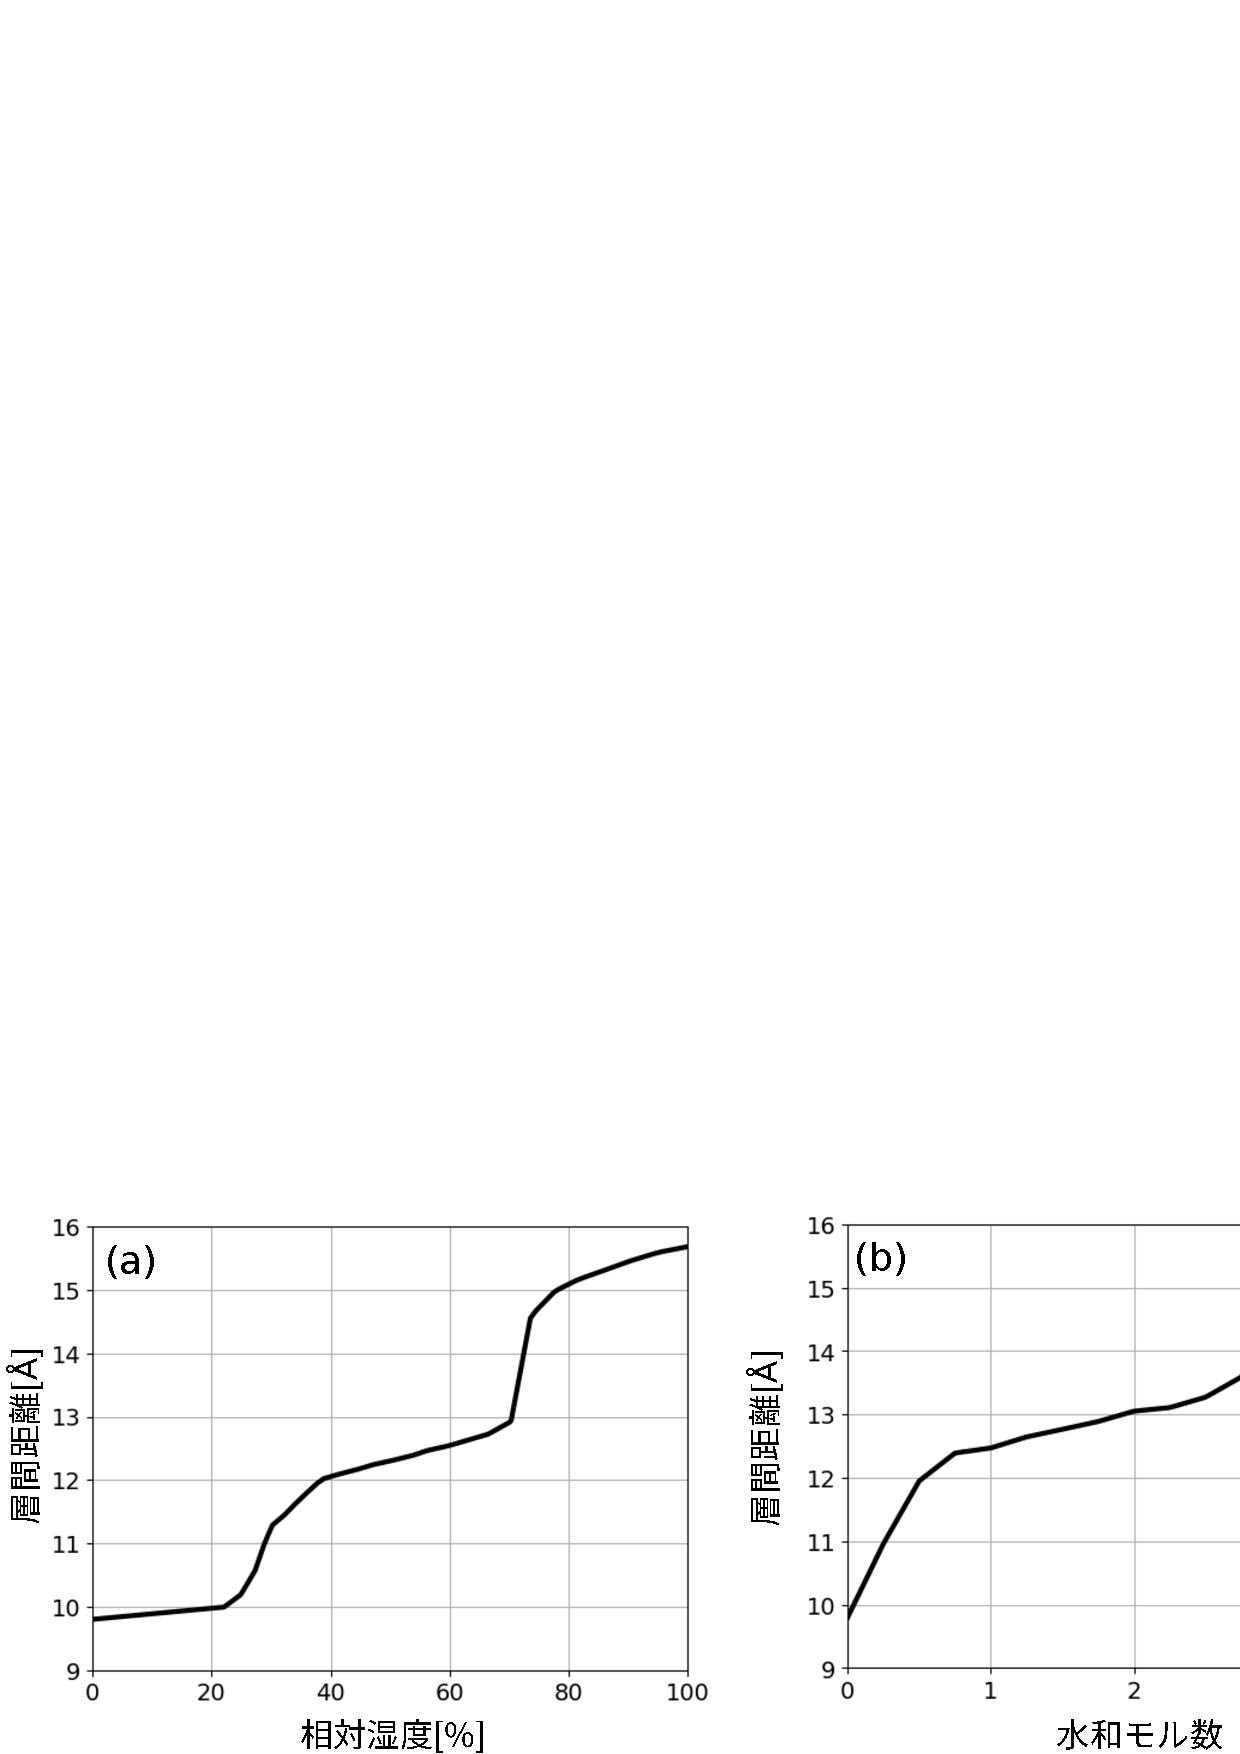
\includegraphics[width=1.0\linewidth]{Figs/fig1.pdf} 
	\end{center}
	\caption{
		Na型モンモリロナイトの膨潤挙動.
		(a)粉末X線回折試験で得られた相対湿度と層間距離の関係(諸留,河村\cite{Morodome}から再現).
		(b)全原子分子動力学計算で得れられた水和モル数と層間距離の関係(森本ら\cite{Morimoto}の
		データを使用). 
	} 
	\label{fig:fig1}
\end{figure}
これに加えて層間距離\(h\)と水分子数\(N\)の関係が得られば,
二つの関係をあわせて\(r_H\)と\(N\)の関係が定められる.
%式(\ref{eqn:mu_hyd})の両辺を\(N\)あるいは\(r_H\)に変数を統一して書くことができる.
そこで,層間距離$h$と水和モル数\(n\)の関係:
\begin{equation}
	h=h(n)
	\label{eqn:hz_nw}
\end{equation}
を全原子分子動力学計算で求める.
図\ref{fig:fig1}-(b)は,森本ら\cite{Morimoto}が行った全原子分子動力学計算の結果を,
$0\leq r_H \leq 1$で観測される層間距離範囲でプロットしたものである.
これら図\ref{fig:fig1}の結果を用い,式(\ref{eqn:hz_nw})と式(\ref{eqn:hz_rh})
を合成してその逆関数
\begin{equation}
	r_H=r_H(n)=r_H(h(n))
	\label{eqn:rh_nw}
\end{equation}
を数値的に求めると,図\ref{fig:fig6}が得られる.
%--------------------
\begin{figure}[h]
	\begin{center}
	\includegraphics[width=0.6\linewidth]{Figs/fig6.pdf} 
	\end{center}
	\caption{
		XRD測定結果\(h=h(r_H)\)と全原子分子動力学計算結果の\(h=h(n)\)
		から得られた,相対湿度$r_H$と水和モル数$n$の関係.
	} 
	\label{fig:fig6}
\end{figure}
%--------------------
式(\ref{eqn:mu_hyd})は任意の平衡状態で成り立つため,粉末X線回折試験
から得られた式(\ref{eqn:rh_nw})を用いれば,次項で示すように,水和エネルギー
を求めることができる.
\subsection{水和エネルギー}
式(\ref{eqn:rh_nw})を式(\ref{eqn:mu_hyd})に代入し,
\begin{equation}
	N=nN_A, \ \ (N_A=6.023\times 10^{23}:アボガドロ数)
	\label{eqn:}
\end{equation}
であることを考慮すれば,式(\ref{eqn:mu_hyd})の変数を\(n\)に統一した次の関係が得られる.
\begin{equation}
	\frac{d G_{hyd}}{d n}
	=
	\mu_w^{sat}N_A +k_BN_AT \log \left\{ r_H(n) \right\}
	\label{eqn:mu_hyd_n0}
\end{equation}
式(\ref{eqn:mu_hyd_n0})で,\(\mu_w^{sat}N_A\)は化学ポテンシャルを1molあたりの
エネルギーとして表したもので,\(k_B N_A\)は気体定数\(R\)に等しい.
そこで,これ以後,化学ポテンシャルの単位はJ/molであるとして,
式(\ref{eqn:mu_hyd_n0})から\(N_A\)を省略すれば,
\begin{equation}
	\frac{d G_{hyd}}{d n}
	=
	\mu_w^{sat} +RT \log \left\{ r_H(n) \right\}
	\label{eqn:mu_hyd_n}
\end{equation}
と書くことができる.ここで,式(\ref{eqn:mu_hyd_n})を温度一定のもと相対湿度$r_H=1$から
積分すれば,自由エネルギー変化:
\begin{equation}
	\Delta G_{hyd}(n) = G_{hyd}(n)-G_{hyd}(n_{sat})
	\label{eqn:del_G}
\end{equation}
が
\begin{equation}
	\Delta G_{hyd}(n)
	=
	\mu_{sat}\Delta n
	+
	RT
	\int_{n_{sat}}^{n} \log \left\{ r_H(n)\right\} dn, \ \ (0 \leq n \leq n_{sat})
	\label{eqn:del_G_mu}
\end{equation}
で計算できる. ただし,\(n_{sat}\)は相対湿度\(r_H=1\)のときに粉末状の粘土がもつ
層間水量を,\(\Delta n\)はその増分
\begin{equation}
	\Delta n = n-n_{sat}
\end{equation}
を意味する. また,粘土含水系の化学ポテンシャルは
\begin{equation}
	\mu(n)
	=
	\frac{d G}{d n}
	=
	\frac{d G_{hyd}}{d n}
	=
	\mu_w^{sat} +RT \log \left\{ r_H(n) \right\}
	\label{eqn:mu_system}
\end{equation}
となる.式(\ref{eqn:mu_system})において$\mu_w^{sat}$は定数だから,
層間水量による化学ポテンシャルの変化は右辺の対数項で与えられ,
この項が層間イオン種に固有の膨潤特性を表現する.また,対応する
自由エネルギー変化は,式(\ref{eqn:del_G_mu})最右辺の積分項で,
最右辺第1項の\(n\)に関する線形項は,層間イオン種毎の特徴とは
関係しない.そこで,
\begin{equation}
	\delta \mu = \mu-\mu_{w}^{sat}
	=
	RT \log \left\{ r_H(n)\right\}
\end{equation}
\begin{equation}
	\delta G_{hyd} =
	RT
	\int_{n_{sat}}^{n} \log \left\{ r_H(n)\right\} dn
\end{equation}
として,これらの\(n\)に対する変化を描くと,図\ref{fig:fig2}の結果が得られる.

%--------------------
\begin{figure}[h]
	\begin{center}
	\includegraphics[width=1.0\linewidth]{Figs/fig2.pdf} 
	\end{center}
	\caption{
		Na型モンモリロナイトの膨潤データから作成した水和エネルギーモデルの特徴.
		(a)化学ポテンシャルの対数項$\delta \mu(n)$, (b)$\delta \mu(n)$に対応する
		水和エネルギー成分$\delta G_{hyd}(n)$.
	} 
	\label{fig:fig2}
\end{figure}
%--------------------

\section{数値解析例}
本節では,Na型モンモリロナイトに対する水和エネルギーを用いて行った
CG-MDシミュレーションの結果を示す.ここでは,非平衡状態にある
モンモリロナイト含水系(以下,単に粘土含水系と呼ぶ)の初期モデルから,
温度,相対湿度,圧力を一定に保った緩和計算を行う.
これを6つの異なる相対湿度において行い,層間距離や粘土分子配置の変化を調べる.
以下では,初期モデルの準備を含む計算手順を述べた後,シミュレーション結果を
粘土分子配置のスナップショットと層間距離の頻度分布として示す。
これらの結果をもとに,相対湿度に応じて組織構造にどのような差が見られるかを述べる.
\subsection{初期モデルの作成}
初期モデルを図\ref{fig:fig3}-(a)に示す.
これは2021年度の共同研究報告書で述べた方法で作成した
粘土含水系モデルの一つである.粘土含水系を構成する
分子数は80で,合計の粗視化粒子数は3,194となっている.
このモデルは以下の計算を経て得られたものである.\\
\hspace{\parindent}
はじめに,直線状の粘土分子を200$\times$200[nm$^2$]の矩形領域に,
互いに重ならないよう,位置と向きをランダムに配置する.
この矩形領域を周期構造の単位セルとして,乾燥密度が約1.6g/cm$^{3}$
となるまで断熱圧縮する.その際,粒子系の運動方程式を積分するための
時間ステップ幅は0.02[ps],時間ステップ数は5万ステップ,
時間範囲は1[ns]としており,時間ステッピングに関する
条件は以後の解析でも同じである.断熱圧縮過程では,
系の温度を制御しないため,圧縮によってに加えれられたエネルギーで
粘土含水系モデルは高い温度となり平衡状態にも無い.
そこで,圧縮後のモデルを300Kまで$250$psの間冷却し,
その後750ps温度を300Kに保ってで緩和計算を行う.
なお,ここでいう緩和とは,温度や体積などの外的条件を一定にして
系を平衡状態へ推移させることを意味する.
以上の計算では,各粗視化粒子が保持する水分量を表すパラメータである
粒子間相互作用ポテンシャルの特性距離$\sigma$は,
二層膨潤状態に相当する$\sigma=1.5$[nm]に固定している.
これは,系内での水分移動も系外との水分の授受も行わない
ことを意味する.最後に,無次元化された化学ポテンシャル$\bar \mu$
を$0.5$に保ち,温度,体積一定のもと,水分移動を許容した
緩和計算を1ns間行う.このとき$\bar \mu$の値は強い排水が起こるように
設定されているため,緩和計算後は,比較的大きな層外空隙をもつ
組織構造が得られる.\\
\hspace{\parindent}
図\ref{fig:fig3}-(a)は,以上の方法で得られた粘土含水系モデルである.
本年度の研究では,これを初期構造とし,Na型モンモリロナイトの
水和エネルギーモデルを用いて,相対湿度一定での緩和計算を行う.
なお,初期構造を得るまでの計算では,昨年度の研究で検討した
水和エネルギーモデルの一つである振動モデルを用いている.
このモデルは仮想的な粘土の水和挙動を表現したものであるため,
図\ref{fig:fig3}-(a)の状態は,今回新たに作成した水和エネルギー
モデルの下では平衡状態にない.そのため,相対湿度の設定値によらず,
水分や分子配置には必ず何らかの変化が生じる.
%%%%
\subsection{相対湿度50$\%$に対する結果}
図\ref{fig:fig3}の(b)と(c)は,相対湿度50$\%$,温度300K, 圧力10MPaで
1ns間,緩和計算を行ったときの粘土分子配置の変化を示したものである.
(b)は経過時間が250psの時点での配置を,(c)は1nsで緩和計算を終了した
時点の結果を示している.
初期状態(a)では水分量が少ないため,緩和計算初期の段階で速やかに
吸水が起こり,(b)では積層間隔が拡がった結果,A-Dのラベルで示した
層外間隙の量が(a)よりも減少している.
一方,(b)から(c)の間には,粘土分子の配置にあまり大きな変化は
なく,(b)の時点から安定した構造が形成されていることがうかがわれる.
ただし,間隙Aの収縮は(b)から一層進行し,(c)の図ではほぼ消失している.
これに対して,粘土分子を巻き込むことで形成された層外間隙の
CとDは,吸水に伴う層間距離の拡張で生じる収縮は比較的小さく,
水分量の変化に対し組織構造を維持する役割を果たしていると推察される.
また,この計算では領域全体の体積は拘束されていないため,
初期状態(a)から(b)を経て(c)に移行する過程で,若干全体としての
体積収縮が認められる.このように,吸水による層間距離の拡張がある場合も,
層外間隙の収縮が勝り,全体としては収縮がおきることもあり得る点は,
マクロスコピックな膨潤挙動について考える際にも留意すべき点と考えられる.
%--------------------
\begin{figure}[t]
	\begin{center}
	\includegraphics[width=1.0\linewidth]{Figs/fig3.pdf} 
	\end{center}
	\caption{
		相対湿度50$\%$での緩和にともなう粘土分子配置の変化.  
		(a)は初期状態,(b)緩和開始から200psの状態,(c)は1ns経過後の最終状態.
		A-Dのラベルは粘土層外の主要な間隙を示す.
	} 
	\label{fig:fig3}
\end{figure}
%--------------------
\begin{figure}[h]
	\begin{center}
	\includegraphics[width=0.7\linewidth]{Figs/fig4.pdf} 
	\end{center}
	\caption{
		6つの異なる相対湿度において得られた粘土含水系の組織構造.
		相対湿度は(a)から(f)の順に10,20,50,65,75および90$\%$. 
		相対湿度50$\%$の結果は,図\ref{fig:fig3}-(c)と同じものを再掲.
	} 
	\label{fig:fig4}
\end{figure}
\subsection{相対湿度による組織構造の違い}
ここまでに示した相対湿度50$\%$の場合に加えて,
10,20,65,75および90$\%$で緩和計算を行った結果を
図\ref{fig:fig4}に示す.なお,これらの計算において,
相対湿度以外の計算条件は前項50$\%$の場合と同じである.\\
\hspace{\parindent}
図\ref{fig:fig4}のうち,相対湿度が最も低い(a)10$\%$の
ケースでは,初期構造(図\ref{fig:fig3}-(a))からあまり
変化がなく,層外間隙の形や大きさはも当初と同程度の
ままになっている.これは,初期構造が相対湿度$10\%$程度の
低い場合に生じるものであったことを意味する.
ただし,系全体の体積はやや初期状態から収縮しており,
若干の排水が生じていることが予想される.2番目に低い
相対湿度である(b)20$\%$では,全体体積は(a)と同程度の
収縮を起こしている.また,初期構造から大きく収縮する
層外間隙もあり,相対湿度50$\%$(図\ref{fig:fig3}-(c)と図\ref{fig:fig4}-(c))
によく似た分子配置となっている.
ただし(c)$50\%$のケースと比べると,初期状態からの
系全体の収縮量は(b)の方が大きく,(b)から(c)の
相対湿度範囲では次第に吸水の効果が大きくなりつつある
と解釈できる.これに対して(d)65$\%$の場合,
全体としての体積変化はほぼ無視できる程度だが,
粘土層間の距離は(b)や(c)の場合より大きく,
吸水による膨張の効果が系全体に及びはじめている.
この段階では粘土分子の巻き込みで残留した層外空隙も
かなりの程度圧縮が進んでいる.さらに相対湿度の高い
(e)75$\%$と(f)90$\%$では,系全体としても膨張し始め,
このことは,層外間隙の体積収縮が(d)のケース
以上には大きく進行しないことと呼応している.\\
\hspace{\parindent}
相対湿度と膨潤状態の関係をより詳しく調べるために,
層間距離の相対湿度による変化をみる.
図\ref{fig:fig5}はその目的のために,
層間距離の頻度分布を相対湿度毎に示したものである.
これらのグラフは,横軸が層間距離を縦軸が頻度を示している.
CG-MD法では,粒子間相互作用を規定するレナード-ジョーンズ
ポテンシャルの特性距離$\sigma$で水分量を表現している.
$\sigma$は,概ね,粘土分子が積層したときの層間距離となるため,
$\sigma$を層間距離とみなし, その頻度分布を描いたのが
図\ref{fig:fig5}である. 横軸の範囲は,10から16$\AA$としており,
縦軸はグラフ毎に適切なサイズに描画されるように設定している.
なお,図\ref{fig:fig1}-(a)にもあるように,系が気体状態の水
に接している状態では,これらの頻度分布に示した範囲外の
層間距離となることはない.また,無水状態である0膨潤で
層間距離は約10$\AA$,1および2層膨潤状態では,層間距離は
それぞれ12.5と15.5$\AA$である。ただし,図\ref{fig:fig1}-(a)から
も分かるように,天然のモンモリロナイトでは,0から2層までの
膨潤状態それぞれに対応す層間距離を厳密に定義することは難しく,
上に挙げた層間距離は代表値と考えることがより実情にあう.\\
\hspace{\parindent}
図\ref{fig:fig5}に示されるように,全体としては
相対湿度の増加にともない,頻度分布の山は右方向に移り
層間距離が大きくなる傾向があることは明らかである.
ただし,分布幅と形状は相対湿度によって異なり,
相対湿度が低いときと,複数のピークが現れる場合に
分布幅が大きくなる傾向がある.
また,一つ一つ相対湿度における分布に関しては,以下のことが読み取れる.\\
\hspace{\parindent}
相対湿度が最も低い(a)の結果は,他の場合と比べて分布幅が明らかに広い.
このとき,層間距離は10$\sim$12$\AA$の間に分布し, 0層と1層膨潤の
中間的な状態になっている.2番目に相対湿度の低い(b)では,層間距離が
12$\AA$周辺に集中し,ほぼ1層膨潤状態に移行している.
図\ref{fig:fig1}-(a)を見ると,粉末X線回折試験では10$\sim$20$\%$の
相対湿度では層間距離は10$\AA$の0層膨潤となっているため,
CG-MD計算の方がより多くの水分が保持される結果となっている.
これは,(a)の状態から更に排水を進めるためには,すでに形成されている
粘土分子の積層構造を変形させる必要があるが,粉末状態の粘土と比べ
変形を生じさせるためにより多くのエネルギーが必要とされる
ことに起因したものと考えられる.
%狭い領域で積層した状態では変形が起こりにくく,水分を持つ方が,系全体の
%自由エネルギーを下げ,構造を安定させるためと考えられる.
%逆に言えば,指定された初期構造から0層膨潤状態に移行させるためには,
%より大きなエネルギーを加えて計全体を強く圧縮するか,組織構造
%を破壊する必要があることを示唆している.
これに対し,相対湿度50$\%$の結果(c)では,分布幅が狭く
層間距離がほぼ12.5$\AA$と決まる.この層間距離は粉末XRD試験の結果
と一致している.また,系全体としても体積膨張を起こすことなく水分が
取り込まれていることから,初期構造から到達および維持されやすい組織構造
になっていると考えられる.次に,(d)65$\%$と(e)75$\%$の結果を見ると,
3つあるいは2つピークをもつ多峰分布になっている.
粉末X線試験結果(図\ref{fig:fig1}-(a))をみると,これらの相対湿度は
1層から2膨潤への遷移領域にあたっている.
頻度分布における13$\AA$と15.5$\AA$付近のピークは,1層および2層膨潤
にそれぞれ対応している.14$\AA$付近にはピークが無いことから,
1層と2層膨潤が混在しているものの,中間的な膨潤状態は現れておらず,
Na型モンモリロナイトの離散的な膨潤挙動がシミュレーション結果に現れている.
ただし,(d)の結果では13$\AA$前後で大小2つのピークに分布が分離している.
大ピークは安定な1層膨潤状態にとどまっている層間水を,
小ピークは,既に2層へ移行が開始しつつあるものの,十分な水分が行き渡らず
1層膨潤に近い層間距離にとどまる箇所があることを意味している.
実際,大小のピークの谷間である13.1$\AA$は,図\ref{fig:fig1}-(a)に
ある膨潤曲線が大きく折れ曲がっており,この層間距離を境に,粉末試料でも
膨潤挙動が変化している.このことを踏まえれば,(d)よりやや相対湿度の
高い(e)で大ピークが消失していることは,全ての層間水が2層膨潤状態に
向かって移行を開始した状態にあると解釈できる.
最後に,最も相対湿度の高い(f)の場合は、2層膨潤への移行が終了し,
鋭いピークを持つ分布が現れている.そのピーク位置は15.5$\AA$で,
粉末X線回折試験結果で観察される層間距離とほとんど一致している.\\
\hspace{\parindent}
%なお,(d)に見られる第3の小ピークを伴う遷移挙動が実際の固体粘土で観察も
%現れるのか,
以上のように,今回のCG-MD計算に用いた水和エネルギーモデルでは,
1層から2層膨潤へは,Na型モンモリロナイトの粉末X線回折試験結果に見られる
離散的な膨潤挙動がよく現れている.
一方,湿度の低いケースでは,0層膨潤状態ははっきりと現れず,1層から0
層膨潤への移行が粘土分子の積層構造に妨げられる可能性があることが分かった.
このような挙動が実際の粘土でも現れるのか,またその影響がX線回折パターン
にも反映されるかは,メソスケール組織構造を実験によって調べる上で
興味深い問題の一つと思われる。
%--------------------
\begin{figure}[h]
	\begin{center}
	\includegraphics[width=1.0\linewidth]{Figs/fig5.pdf} 
	\end{center}
	\caption{
		6つの異なる相対湿度における層間距離の頻度分布.
		相対湿度は(a)から(f)の順に10,20,50,65,75および90$\%$. 
		(c)に示した緑の分布は,初期構造(緩和計算開始時)の
		層間距離の頻度分布を表す.
	} 
	\label{fig:fig5}
\end{figure}
%--------------------

\section{まとめと今後の課題}
本研究では,相対湿度を指定したCG-MD計算を行うプログラム機能の追加を行った.
その結果,温度や湿度,圧力,体積など,実験で制御することのできるマクロ変数
を指定したCG-MDシミュレーションが可能となった.
%これは,X線回折試験や膨潤試験時の実験条件に対応させたCG-MDシミュレーションが可能となったことを意味する. 
さらに,X線回折試験と全原子分子動力学計算で得られた膨潤曲線を用いて
水和エネルギーモデルを設定する方法を提案した.以上により,実験で観測される粘土の
膨潤特性を水和エネルギーを介してCG-MD計算に反映し,組織構造形成や吸排水に
よる膨潤のシミュレーションを行うプログラム機能が整えられた.
%
開発したプログラムを使った数値解析例では,
Na型モンモリロナイトを想定した水和エネルギーを用い,
$10\%\sim 90\%$の6つの異なる相対湿度で
どのような組織構造が形成されるかを調べた.
%その結果,相対湿度の上昇に伴い,吸水による層間距離の 拡張が起き,
%低い相対湿度では層外間隙が次第に収縮し,高い相対湿度ではそれに
%加えて系全体が体積膨張を起こす様子が見られた.
%また,層間距離の頻度分布を相対湿度毎に調べたところ,
その結果,20$\sim$90$\%$の広い相対湿度の範囲で,
1層あるいは2層膨潤状態が明確に現れること,
これら2つの膨潤状態が混在する場合はあるが,
両者の中間的な膨潤状態はCG-MD計算結果に現れな
いことが分かった.
%さらに,相対湿度が50$\%$以上の場合,層間距離は粉末X線回折
%試験で得られる結果と概ね一致し,Na型モンモリロナイトの膨潤特性を
%よく表現することが分かった.
一方,相対湿度が10$\sim$20$\%$の範囲では,0層膨潤への明確な移行は見られず,
粉末X線回折試験と異なる結果となった.
これは,粘土が密な積層構造を作ることに起因した挙動と予想されるが,
実際に生じる現象であるか否かは知られていないため,
今後実験との比較で検証していく必要がある.
%そのためには,例えば,シミュレーション結果から合成したX線回折パターンを
%実測値と比較することが有効な方法になると考えられる.
\\
%
\hspace{\parindent}
CG-MD法やその前提となるモデルの妥当性を検証するには,
観測可能なマクロ量をシミュレーション結果から算出して実測値と比較する
ことが必要となる.そのような検証を経てシミュレーションの妥当性が確認
できれば,X線回折試験結果をはじめ,実験データの解釈にCG-MD
シミュレーションを利用することも可能になる.現状,ナノメートルスケール
の多孔質構造を湿潤状態でその場観測する手法はなく,粘土含水系の組織構造
には不明な点が多い.そのため,信頼性のある組織構造モデルを生成可能な
シミュレーション技術を開発することは,粘土含水系のメソ,マクロ物性と
組織構造の関係を理解する上で重要である.CG-MD法はその基礎技術となりうる
ことが期待されるが,十分な信頼性と汎用性をもつためには,引続き,
以下のような課題に取り組む必要がある.
\begin{itemize}
%開発
\item
	CaやKなど各種交換性陽イオンに対する水和エネルギーのモデル化
\item
	X線回折試験をはじめとする実験結果との比較によるシミュレーション
	の妥当性検証とモデルパラメータの最適化
\item
    	3層膨潤以上の状態を扱うための水和エネルギーモデル開発と,
	その基礎となるX線回折データの取得
\item
	並列化可能箇所の抽出と, 高速アルゴリズムの適用による
	計算効率の改善.大規模計算の実施ならびに3次元モデルへの拡張.
\item
	平衡状態における水分分布の安定性評価と非定常水分浸透解析への応用
%\item
%	水和エネルギーとの独立性が保証される粒子間相互作用ポテンシャルの導出
%\item
%	水分拡散係数を求める方法を開発すること(弱い非平衡系への拡張)
%\item
%	モデルパラメータの最適化.例えば,運動方程式の時間ステッピングに
%	対する,水分移動に関するモンテカルロ計算の頻度を合理的な設定.
%\item
%	並列化可能箇所の抽出, 高速アルゴリズムの適用可能性を検討すること.
%	モンテカルロ法の高速化(サンプリング法の改善)
%検証
%\item
%	粉末XRD回折試験で得られた膨潤曲線のCG-MD法モデルによる正確な再現
%\item
%	実験データとの比較によるモデルおよびシミュレーション法の妥当性検証. 
%	特に,CG-MD計算に基づくX線回折パターンと測定結果の比較.
%	X線回折パターンから推定可能なメソスケール組織構造の有無を調べること.
%\item
%	吸水-排水,膨潤-収縮サイクルにともなう組織構造のヒステリシスについて調べること
\end{itemize}
今後これらの課題を解決することができれば,層間イオン種に応じた不飽和水分浸透や
膨潤解析を行うことで,ベントナイト緩衝材の物質輸送特性の
解明にも貢献しうると考えられる.
\begin{thebibliography}{99}
\bibitem{Eb2014}
	D. Ebrahimi, A. J. Whittle, and R. J.-M. Pellenq, 
	"Mesoscale properties of clay aggregates from potential of mean force representation of
	interactions between nanoplatelets",
	The Journal of Chemical Physics 140, 154309, 2014. 
\bibitem{Eb2016}
	D. Ebrahimi, R. J.-M. Pellenq, A. J. Whittle,
	"Mesoscale simulation of clay aggregate formation and mechanical properties",
		Granular Matter vol.18(49), 2016.
\bibitem{Katti}
	D. R. Katti, M. I. Matar, K. S. Katti, and P. M. Amarasinghe, 
	"Multiscale modeling of swelling clays: a ccmputational and experimental approach, 
	KSCE Journal of Civil Engineering, vol.13(4), pp.243-255, 2009.
\bibitem{Tombach}
	T. J. Tambach, P. G. Bolhuis, E. J.M. Hensen, and B. Smit, 
	"Hysterisis in clay swelling induced by hydrogen bonding: 
		Accurate prediction of swelling state, Langmuire, 
	vol.22, pp.1223-1234, 2006.
\bibitem{Morodome}
	S. Morodome and K. Kawamura, 
	"Swelling behavior of Na- and Ca-montmorillonite up to 150°C by 
	in situ X-Ray diffraction experiments", 
	Clays and Clay Minerals,vol.57, pp.150-160, 2009.
\bibitem{Yamada}
	H. Yamada, H. Nakazawa, H. Hashizume, S. Shimomura, and T. Watanabe, 
	"Hydration behavior of Na-smectite crystals synthesized at high pressure 
	and high temperature, Clays and Clay Minerals, vol.42, No.1, pp.77-80, 1994.
\bibitem{Morimoto}
	森本 逸紀,木本 和志,河村 雄行,
	"分子動力学法によるモンモリロナイト層間の水分子と陽イオンの分布解析", 
		土木学会論文集A2(応用力学), vol.78, 2022(掲載決定). 	
\end{thebibliography}
\end{document}
%%%%%%%%%%%%%%%%%%%%%%%%%%%%%%%%%%%%%%%%%%%%%%%%%%%%%%

